\subsection{Formalization}

%---lane events
\begin{figure}% >>>
  \centering
  \begin{minipage}[t]{.363\linewidth}
    {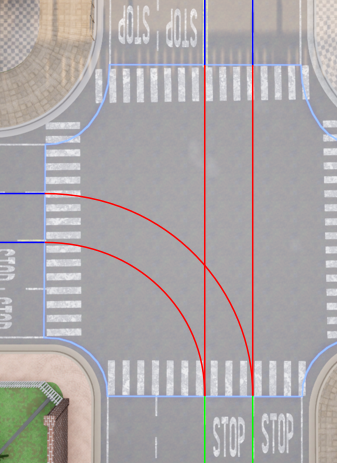
\includegraphics[width=\linewidth]{figures/chapter4/lanes-south.png}}%
    \subcaption{Incoming, connecting, and outgoing lanes (green, red, blue).}
  \end{minipage}%
  \hfill
  \begin{minipage}[t]{.3\linewidth}
    {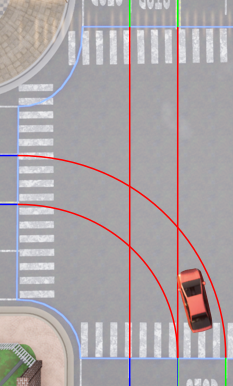
\includegraphics[width=\linewidth]{figures/chapter4/lanes-enter.png}}%
    \subcaption{A car entering a lane that intersects its route (left turn).}
  \end{minipage}%
  \hfill
  \begin{minipage}[t]{.3\linewidth}
    {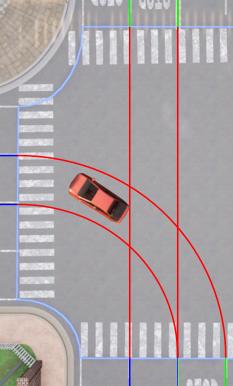
\includegraphics[width=\linewidth]{figures/chapter4/lanes-exit.png}}%
    \subcaption{A car exiting a lane that intersects its route (left turn).}
  \end{minipage}%  
  \caption{Lane events.}
  \label{fig:lane-events}%
\end{figure}% <<<


We use Python objects to represent a scenario, and reuse the data structures in Scenic's driving domain.\footnote{\url{https://scenic-lang.readthedocs.io/en/latest/libraries.html##driving-domain}}
%
The traffic rules are modeled as first-order logic sentences over the elements, attributes, states, actions, events, etc. in a scenario.
%
These sentences are represented in a logic program, more specifically an Answer Set Program.
%
In this section we explain some of the details.


%---scenery
The scenery is modeled as a road network in Scenic's driving domain.
%
A road \emph{network} is a collection of \emph{roads} and \emph{intersections}.
%
An \emph{intersection} connects two or more \emph{roads} together.
%
Each \emph{road} is a collection of \emph{lanes} and posted \emph{signs}.
%
A \emph{lane} is a polygonal region of the road together with an associated driving direction.
%
A lane is either a part of a road or a part of an intersection.
%
The \emph{incoming} lanes of an intersection are the road lanes that end at that intersection.
%
The \emph{outgoing} lanes of an intersection are the road lanes that start at that intersection.
%
The \emph{connecting} lanes of an intersection are intersection lanes that connect an incoming lane to an outgoing lane.
%
A \emph{route} is a triple of (incoming, connecting, outgoing) lanes at an intersection.
%
See Figure~\ref{fig:lane-events} for (a) two routes from the same incoming lane, and (b) two routes from different incoming lanes.
%
The connecting lanes are polygonal regions even though their boundaries appear smooth.


%---dynamic elements
A car has attributes such as shape, wheelbase, maximum steering angle, etc.
%
Scenic models the \emph{shape} of a car as a rectangle, which simplifies computing the lane events (entrance and exit).
%
The \emph{location} of a car is the location of the center of its rectangle.
%
The \emph{state} of a car in a scene specifies its \emph{pose} (location and orientation) and turn signal.
%
The \emph{behavior} of a car is the sequence of its states at each scene.
%
When the shape of a car starts overlapping a lane, it \emph{enters} the lane, and when it stops overlapping, it \emph{exits} the lane.
%
See Figure~\ref{fig:lane-events}.


%---traffic rules
The traffic rules describe right-of-way rules and abiding by traffic signs.
%
We model the traffic rules in an Answer Set Programming (ASP) language similar to~\cite{Karimi.2020}.
%
Before presenting our formulation, we need a quick introduction to ASP.
%
An ASP \emph{program} is a collection of \emph{rules} of the form:
\begin{center}
\clingo{h :- p_1, ..., p_n, not p_{n+1}, ..., not p_{n+m}.}
\end{center}
%
We call \clingo{h} the \emph{head} of the rule, and the list after \clingo{:-} is the \emph{body} of the rule.
%
The intended meaning of the above rule is
$$ p_1 \land \dots \land p_n \land  \neg p_{n+1} \land \dots \land \neg p_{n+m} \rightarrow h $$
%
Here each \emph{condition} $p_i$, as well as $h$, is an \emph{atomic predicate} over constants and variables.
%
An atomic predicate or a rule is \emph{ground} if it has no variables.
%
A \emph{fact} is a ground rule with no conditions.
%
A rule is used to infer more facts, except if the head is empty.
%
If the head is empty, we get a \emph{constraint} which means that the conjunction of predicates $p_1 \ldots \neg p_{n+m}$ should not hold true.
%
A \emph{choice rule}, which is a syntactic sugar, is a rule where the head is a list of predicates to choose from.
%
In particular,
\begin{center}
\clingo{{ h_1, ..., h_k } = N :- p_1, ..., not p_{n+m}.}
\end{center}
specifies that exactly \clingo{N} predicates from the list \clingo{h_1, ..., h_k} must be inferred if the body of the rule is true.
%
The domains of variables are determined using Herbrand semantics \cite{Herbrand.2019}, that is from all the constants mentioned in the program.
%
Given an ASP program, the ASP solver finds a set of facts (i.e. an \emph{answer set}) that is closed under the rules of the program.
%
If no such set exists, the ASP solver returns that the program is \emph{unsatisfiable}.



%---examples
Relations, actions, events, etc. in a scenario are included in an ASP program as facts.
%
For example, if the incoming lane \clingo{road8_lane0} has a stop sign, we represent this with a fact  \clingo{hasStopSign(road8_lane0)}.
%
The event of \clingo{car1} arriving at the intersection at time \clingo{t1} from the incoming lane \clingo{road8_lane0} is represented by the fact 
\begin{center}
\clingo{arrivedAtForkAtTime(car1, road8_lane0, t1)}.    
\end{center}
%
Here, \emph{fork} is an incoming lane together with its connecting lanes.
%
Traffic rules are added to a program to infer the violations.
%
For example, to infer the violations of the traffic rule \emph{``the driver of any vehicle approaching a stop sign at the entrance to an intersection shall stop''} we add
\begin{minted}[fontsize=\small]{prolog}
violatedRule(V, stopAtSign) :-
  arrivedFromIncomingLane(V, L), hasStopSign(L),
  not stoppedAtIncomingLane(V, L).
\end{minted}
%
Here, \clingo{violatedRule(V, stopAtSign)} is an atomic predicate that can be inferred to be true or false based on the grounding of variables \clingo{V} and \clingo{L}, and the truth of the rule's conditions.
%
Traffic rule violations are found simply by checking whether the answer set includes a corresponding fact.
%
In our formalization, we have two types of violations: \clingo{violatedRule(V, r)} and \clingo{violatedRightOfForRule(V1, V2, r)}.
%
The first violation involves one vehicle \clingo{V} violating a rule named \clingo{r}, and the second is a violation where vehicle \clingo{V1} violated the right-of-way of vehicle \clingo{V2} according to the traffic rule named \clingo{r}.
%
For example, the rule above is named with the term \clingo{stopAtSign}.
%
Note that upper-case terms are variables and lower-case terms are constants.
%
In the next section, we will see examples of choice rules used to search through possible orders between events, and constraints used to restrict the search space.


%---perceptible temporal order
We use the notion of \emph{perceptible order} to model ordering of events in traffic rules.
%
The parameter \emph{minimum perceptible time difference} is a threshold beyond which events are considered simultaneous from the perspective of traffic rules.
%
Suppose that $m$ represents this parameter, and let $s, t$ be two moments in time.
%
Then $s, t$ are \emph{perceptibly simultaneous} if $|s-t| < m$.
%
Otherwise, $s$ \emph{perceptibly precedes} $t$ or vice versa, if $m \leq t-s$ or $m \leq s-t$, respectively.
%
Perceptible simultaneity is not transitive since $|r-s|<m$ and $|s-t|<m$ do not imply $|r-t|<m$.
%
Therefore, perceptible order is not a partial order.
%
In contrast, \emph{temporal order}, i.e. the standard real number order of time points, is a partial order.
%
Consequently, we use separate binary relations to represent perceptible order and temporal order.

